\chapter{Exemple de structure de données linéaires dynamiques}\label{sdDynamique}
\section{Pile}
Liste simplement chaînée dynamique à un point d'entrée

\begin{figure}[H]
	\centering
	\includegraphics[width=6cm]{content/pile.eps}
	\caption{Pile avec une liste simplement chainée}
\end{figure}

\begin{lstlisting}[language=C, numbers=none,frame=none, caption=Stucture \texttt{CelSc} -- Pile avec liste simplement chaînée]
	typedef struct etCel {
	Element val;
	struct etCel *suiv;
} CelSc;
\end{lstlisting}

\section{File}
Liste simplement chainée à deux points d'entrée

\begin{figure}[H]
	\centering
\includegraphics[width=6cm]{content/file.eps}
	\caption{File avec une liste simplement chainée}
\end{figure}
\begin{lstlisting}[language=C, numbers=none,frame=none, caption=Structure \texttt{LSC2} -- File avec liste simplement chaînée]
	typedef struct etCel2 {
	LSC fin;
	LSC debut;
} LSC2;
\end{lstlisting}
\section{Pile avec liste doublement chainée}
\begin{figure}[H]
	\centering
\includegraphics[width=12cm]{content/pileDoubleChaine.eps}
	\caption{Pile avec une liste doublement chainée}
\end{figure}

\begin{lstlisting}[language=C, numbers=none,frame=none, caption=Structure \texttt{CelDC} -- Pile avec liste doublement chaînée]
typedef struct etCelDC {
	Element val;
	struct etCelDC* suiv;
	struct etCelDC* precedent;
}CelDC;
typedef celDC* LDC;
\end{lstlisting}

\section{File avec liste doublement chaîné}
\begin{figure}[H]
	\centering
\includegraphics[width=12cm]{content/fileDoubleChaine.eps}
	\caption{File avec une liste doublement chainée}
\end{figure}
